\documentclass{main}
%----------------------------------------------------------------------------------------
%	Definitions
%----------------------------------------------------------------------------------------
\newcommand{\DefType}{Bachelor Thesis} %Type of your scientific work
\newcommand{\DefTitle}{Modeling and Evaluating CPU Caches in Software} %Title of your work
\newcommand{\DefFirstAuthor}{Mario Theuermann} %Name
\newcommand{\DefFirstAuthorMatnum}{01430751} %Matr number.
\newcommand{\DefFirstAuthorEmail}{mario.theuermann@student.tugraz.at} %Email address
%space for more Authors
%\newcommand{\DefAuthorFront}{\DefFirstAuthor\ \DefFirstAuthorMatnum,\\ \DefSecondAuthor\ \DefSecondAuthorMatnum}
\newcommand{\DefAuthorFrontPage}{\DefFirstAuthor (\DefFirstAuthorMatnum)}

\newcommand{\DefAuthor}{\DefFirstAuthor}
\newcommand{\DefVersion}{1.0}
\newcommand{\DefLogo}{TU_Graz_Logo.pdf}

\begin{document}
\begin{titlepage}
	% --------------------------------------------------------------
	%     Title section & picture
	% --------------------------------------------------------------
	\titlesection{\DefLogo}
	\newcommand{\HRule}{\rule{\linewidth}{0.5mm}} % defines a new command for horizontal lines, change thickness here
	\centering % centre everything on the page
	\vfill \vfill
	
	%------------------------------------------------
	%	Type of scientific document e.g. BS Thesis
	%------------------------------------------------
	\HRule\\[0.4cm]
	{\huge\bfseries\DefType}\\[0.4cm] % Type
	\HRule\\[1.5cm]
	
	%------------------------------------------------
	%	Title of your work e.g. The story of a little fluffball named Heinrich
	%------------------------------------------------
	\textsc{\Large\DefTitle}\\[0.5cm] % Main heading 
	
	\vfill %\vfill
	%------------------------------------------------
	%	Author(s)
	%------------------------------------------------
	%\begin{flushleft}
		\large{
			\DefAuthorFrontPage\\ 	
			\href{mailto:\DefFirstAuthorEmail}{\DefFirstAuthorEmail}\\[0.4cm]
		}
	%\end{flushleft}

	%------------------------------------------------
	%	Date
	%------------------------------------------------
	\vfill\vfill\vfill % Position the date down
	{\large\today} % Date, change the \today to a set date if you want to be precise
	
	%------------------------------------------------
	%	Link
	%------------------------------------------------
	\url{http://www.iaik.tugraz.at/content/teaching/}	
	\vfill % Push the link up 
	
\end{titlepage}
% --------------------------------------------------------------
%     insert last update
% --------------------------------------------------------------
% \lastupdated

% --------------------------------------------------------------
%     abstract
% --------------------------------------------------------------

%\pagebreak
% --------------------------------------------------------------
%     TOC
% --------------------------------------------------------------
% \tableofcontents

\pagebreak
\twocolumn
\sloppy
% --------------------------------------------------------------
%      start document
% --------------------------------------------------------------

\begin{abstract}
	
\textbf{In microprocessor cache architecture design, there is an increasing demand for techniques to model miscellaneous different cache concepts, that enable to investigate the threats of cache-based side-channel attacks. A cache simulation offers many benefits in contrast to hardware testing when studying cache behaviour of modern multi-core microprocessor architectures. Accurate runtime simulations can greatly assist reasearchers to further explore access-driven cache attacks. Therefore a cache simulation enabling a full system emulation of the cache behaviour of x86 virtualization hosts can be advantageous. We present the current status of a runtime cache simulation using the well-known instruction set simulator QEMU, that can serve for research purposes on access-driven cache-attacks. Furthermore, this implementation model is extended to act as a trace-driven cache simulation, modeling and evaluating many different cache characteristics and scenarios.}
	
\end{abstract}

\section{Introduction}

\textit{Side-channel attacks} form a class of implementation level attacks that are of basic interest when it comes to cryptographic systems. Their principle is based on information about the implementation details of a computer system itself. They exploit, for instance, the leakage of information from electromagnetic radiation or power consumption of a device \cite{DBLP:journals/iacr/BangerterGK10}, and timing information of certain instructions, in order to recover secret data such as cryptographic keys. 

Especially side-channel attacks based on cache access mechanisms of modern microprocessors developed a large field of research over the past few years, although some showed other types of cache attacks, such as detecting cryptographic libraries \cite{DBLP:journals/popets/IrazoquiIES15}, bypassing kernel ASLR \cite{DBLP:conf/ndss/HundWH13}, or keystroke logging \cite{DBLP:conf/uss/GrussSM15} as well. \textit{Cache attacks} are definitely one of the most common threats to modern computer systems nowadays. These cache based side-channel attacks can be cassified into three categories: time-driven \cite{DBLP:journals/iacr/Page02} \cite{DBLP:conf/ctrsa/AciicmezSK07}, trace-driven \cite{DBLP:journals/iacr/Page02} \cite{DBLP:conf/wisa/GallaisKT10}, and access-driven attacks \cite{DBLP:journals/iacr/OsvikST05}. 

\pagebreak
The CPU (Central  Processing  Unit) cache itself is a microarchitectural component, which was developed to reduce the amount of slow memory accesses by storing recently used information directly on the processor die. In modern microprocessors, the \textit{last-level cache} (LLC) is accessible from all cores and software can share identical memory pages between processes running on the same system. One example of the purpose of cache-based side-channel attacks (or cache attacks for short) is to retrieve sensitive information by exploiting this shared cache memory. Yuval Yarom and Katrina E. Falkner \cite{DBLP:journals/iacr/YaromF13} showed a cross-core attack, allowing the spy and the victim to execute in parallel on different execution cores called \textit{Flush+Reload}. They extended the famous research by Paul C. Kocher who presented attacks which can exploit timing measurements from vulnerable systems to find Diffie Hellman exponents, factor RSA keys and break other cryptosystems \cite{DBLP:conf/crypto/Kocher96}.

Nowadays a lot of different mechanism are known for attacking the CPU cache such as \textit{Flush+Flush} \cite{DBLP:journals/corr/GrussMW15} and \textit{Prime+Probe} \cite{DBLP:conf/ctrsa/OsvikST06}. There is also a wide variety of different microarchitectural components. Microprocessors for instance feature various hardware specifications that differ in terms of execution speed, bus throughput, hyperthreading options and cache architectures. Evaluating the behaviour of cache attacks using different hardware specifications plays a major role to improve computer security. This paper presents the attempt to simulate cache-based side-channel access-driven attacks using \textit{QEMU}, an open source instruction-level machine emulator \cite{DBLP:conf/usenix/Bellard05}. 

The primary usage of QEMU is to run one operating system (OS) on another \cite{DBLP:conf/usenix/Bellard05}. It is known for its capability to emulate many different guest architectures and CPU types on many different host architectures. Our idea is to modify its complex execution process and change the CPU emulation to provide miscellaneous types of cache architectures, that can simply be simulated and observed on a single host machine. Researchers are interested in measuring, analyzing and improving modern cache management with either empirical studies or simulated analysis. Simulations can enable researchers to change and analyze diverse cache characteristics such as replacement policy, interconnections, and capacity. It can be a tool to analyze this immediate threat to computer security, cache attacks, on a bigger scale although it never will be as realistic as empirical results are. But as a matter of fact, simulation is a key part in testing and evaluating hardware related design improvements. \\

The rest of the paper is organized as follows: First we describe the need of cache memory in general, its development and how it is organized in modern microprocessor architectures nowadays. The principle of shared memory various cache attacks are both important factors of this work. Both are explained in their corresponding sector before we talk about the underlaying concepts of the QEMU machine emulator. The \textit{Methodology}-Section contains contributions to previous topics that arised from this work. Two major simulations are explained: An \textit{On-line simulation} using QEMU that focuses on a runtime cache simulation with a therefore developed cache model and an \textit{Off-line simulation} where this cache model is used to perform trace-driven simulations. Various experiments are evaluated and show the differences of several cache concepts. 

\section{Background}
\subsection{Cache Memory}


The problem is simple and originated from the basic amition of CPU designers to constantly improve their design, increasing processing speed to carry out more instructions in less time, in order to get the highest throughput. This often means they simply increase the CPU clock frequency which increases the number of CPU cycles being performed in a certain time period. It is a big aspect of a processor's performance, but not only the number of cycles being made in the same time is a factor. The average number of instructions per cycle, which is the multiplicative inverse of clock cycles per instruction, is important and differs from one processor architecture to another. 

After a certain point of improving the central processing unit, the system's main memory (DRAM) became the limiting factor in the troughput of a computer system. Concrete, when using DRAM (Dynamic  Random  Access  Memory) with an average access time of about 60ns, CPU designers recognized a drop in terms of throughput when the CPU clock frequency was raised just over 20Mhz. The throughput linearly increases with the clock frequency before it hits this certain point where a processor is not able to operate at its desired speed anymore. A wait state must be inserted for every query with an access time of less than 60ns to account for the difference. By increasing the clock frequency even more, the scalability actually gets worse \cite{DBLP:books/daglib/0092408}. This is illustrated in Figure \ref{fig:troughputvsfreq}. 

\begin{figure}[!ht]
	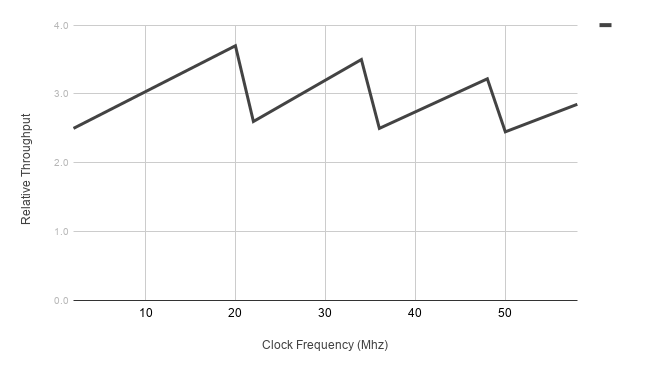
\includegraphics[width=\linewidth]{./figures/throughput_vs_freq_chart1.png}
	\caption{Throughput vs. clock frequency of a typical single-processor system \cite{DBLP:books/daglib/0092408}.}
	\label{fig:troughputvsfreq}
\end{figure}

In a nutshell, while the CPU design evolutionary envolved to serve as a fast instruction worker with lighting reflexes and high clock speeds, DRAM access latency hardly improved over time. This problem can be addressed by applying fast memory to this data processing workflow. However, the limitation of data storage is: The faster, the more expensive per capacity it gets and thus smaller. The principle of dividing the memory space into a faster and slower section was already used in the concepts of a \textit{virtual memory system}. The OS copies portions of code from the slower to the faster portion to ensure that a high amount of the program code executes from a very fast memory and resides in slower, less expensive mass memory when it is waiting to be used \cite{DBLP:books/daglib/0092408}. Processor caches work quite similar with the difference that their contents are completely controlled by hardware logic.  Furthermore, the discovery of the locality principle led to the invention of working sets \cite{DBLP:reference/db/2009} to make use of locality properties that predict upcoming data references and later enabled the design of page replacement algorithms. 

\subsection{Cache Hierarchy}

\begin{figure*}[!ht]
	\centering
	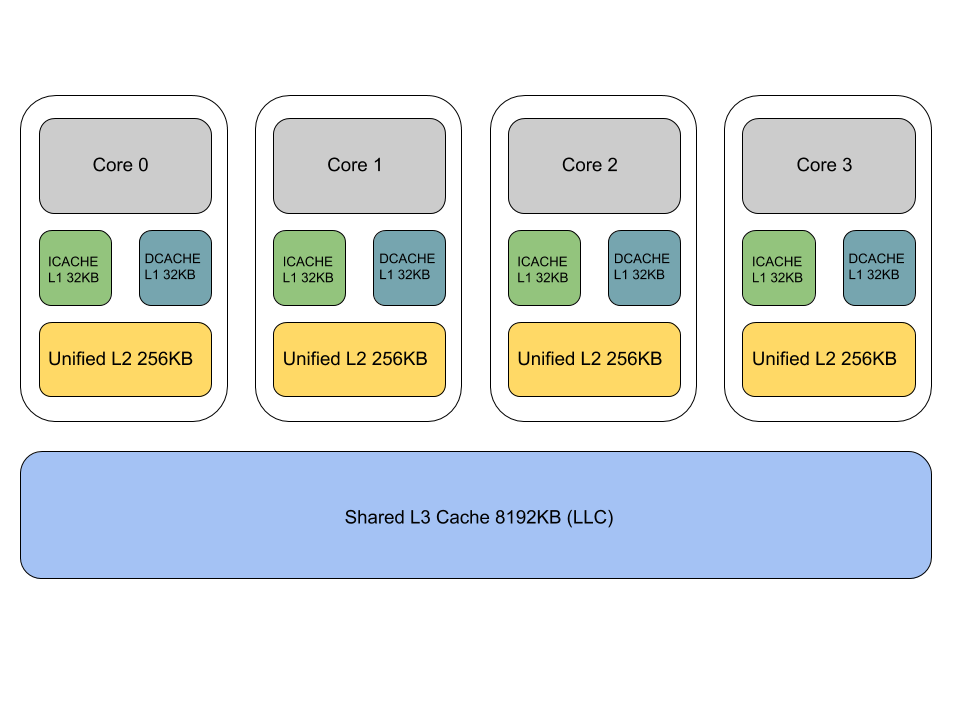
\includegraphics[scale=0.32]{./figures/multilevel_cache_hierarchy_skylake.png}
	\caption{Multilevel cache architecture (Intel Skylake).}
	\label{fig:cachearchitecture}
\end{figure*}

Modern CPU architectures have a hierarchical cache memory structure. Again, this hierarchical structure has economical reasons similar to the difference between DRAM and mass storage devices (e.g.: Hard Disk Drive, Solid State Disk) in virtual memory management. To narrow the exponentially growing performance gap between CPU speed and memory latency, the CPU is composed of multiple cores and lots of hierarchical fast cache memory banks. The speed of the banks increases with less distance to a core and decreases when the distance gets bigger. So in fact, processor caches are designed to bridge the gap between the processing speed of a modern processor and the data retrieval speed of the system's main memory in the most economic way possible. 

Cache memory hierarchies exploit the principle of locality and focus on referencing only small fractions of memory content for given periods of time. Consequently, during each period of time, only the fraction currently referenced, called working set, needs to be present in the fastest memory level, while the remaining data and code can stay in slower levels. In general, all data in one level is also found in all (slower but larger) memory levels below it \cite{DBLP:reference/db/2009}. 

Summing it up, caches store the contents of recently used memory locations, as well as working sets likely to be required by the CPU and evicts working sets decided to not be useful anytime soon, usually by a variation of the \textit{LRU} (Least Recently Used) replacement algorithm. Retrieving data from a cache significantely reduces the pressure on the main memory and saves time. 

A typical modern processor includes three different cache levels as illustrated in Figure \ref{fig:cachearchitecture}, that all resides on the CPU's die. Caches at the top of the hierarchy, typically known as Level 1 or \textit{L1} cache, are the smallest, fastest and nearest to the corresponding processors core. The L1 is split into data and instruction caches on recent Intel processors (32 KiB DCACHE and 32 KiB ICACHE) and has an access time to cached data of 4 CPU cycles. The Level 2 (L2) cache consists of unified data and has a size of 256 KiB and a latency of 7 cycles. In a multicore processor, each of the execution cores has dedicated L1 and L2 caches. The third level cache is called L3 or last-level cache (LLC). It very much varies between specific processor models. For desktop processors the size ranges from 3MiB to 16MiB with a latency of about 35 cycles. Unlike lower-level caches, which are core-private, the LLC is shared between all cores of the processor \cite{DBLP:journals/iacr/YaromGLLH15}. 

Generally, within cache architectures that consists of multiple caches two types must be distinguished that are basically different. \textit{Inclusive caches} always store a replication of data stored in L1 in all upper cache levels, for example L2 and LLC. This means that data fetched from main memory always gets stored in all the cache levels. If a cache line needs to be replaced in L1, which usually is the smallest of all caches, a copy of this data still remains in all higher and thus bigger cache hierarchies. New content can then be loaded from wherever it is found, L2, LCC or main memory. Following the principle of inclusive caches, the full storage capacity of a CPU cache architecture is determined by its largest cache on top of the hierarchy, mostly called LLC. However, it is very important that by definition the LLC contains copies of all the content stored in the lower cache levels. This also means that deleting data from the LLC also removes this data from all lower cache levels. This behaviour is used by various cache attacks since operating systems offer instructions to manipulate the content of the LLC. 

On the other hand, \textit{exclusive caches}, cached data is stored exclusively in one cache level. When fetching memory content it is cached in the lowest level, L1. If a cache line needs to be replaced in L1, it is written to the next level in hierarchy and so forth. Data is written from higher to lower levels with repeated access. Using this principle, the full storage capacity of a CPU cache architecture is the total sum of the single cache level capacities. 

Starting with Intel's \textit{Haswell} microarchitecture another cache level becomes available on various processor models. This \textit{L4} cache uses embedded DRAM (eDRAM) on the same package, as the Intel's integrated GPU \cite{wiki:CPUcache}. This additional cache serves as victim cache to the CPU's on-die LLC cache, which means that this L4 cache hold blocks that were evicted from the LLC cache beforehand. Additionally the L4 allows for memory to be shared dynamically between the GPU and CPU.

\subsection{Cache Mapping}
\label{section:cachemapping}

The important characteristics of caches are: \textit{Cache Capacity} (or \textit{Cache Size}), \textit{Cache Lines}, \textit{Block Size} and \textit{Associativity}. A cache stores fixed-size memory units (defined by the block size) called lines to fully fit its capacity. When the processor issues an access to the main memory, the referenced address, also called main memory address or byte address, first gets mapped into the corresponding cache line. In the most simple case of a \textit{direct} mapped cache with a block size of 1 byte, this may be described as: $cache\_line\_index = byte\_address\ mod\ cache\_size$. Note, that in this particular example the number of cache lines is equal to the cache capacity in bytes. One can also describe this mapping as: $cache\_line\_index = byte\_address\ mod\ cache\_lines$. 

Instead of performing a division, we can resolve the cache line by using the least significant bits $n$ of a memory address that corresponds to the cache size $2^n$. With a cache size of $2^2$ bytes and a block size of 1 byte, the memory address $14$ maps to cache line with index $2$ that contains a data block of 1 byte. The same applies to the memory address six: $6\ mod\ 2^2 = 2$. Table \ref{table:leastsignificant_bits} shows how to determine the cache index of both memory addresses, 6 and 14, using the least significant bits. 

\begin{table}
	\centering
	\begin{tabular}{|c|c|}
		\hline
		Memory address & Cache line index \\ [0.5ex] 
		\hline\hline
		$01{10}_2$ 	& ${10}_2 = 2_{10}$	\\
		$11{10}_2$  & ${10}_2 = 2_{10}$	\\ 
		\hline
	\end{tabular}
	\caption{Calculate the cache index of a memory address using the least significant bits assuming $2^2$ bytes cache capacity and a 1 byte block size.}
	\label{table:leastsignificant_bits}
\end{table}

\textit{Spatial locality} anticipates that an access to one memory address is typically followed by an access to a nearby address. A one byte block size does not take advantage of this observation. Hence, much bigger block sizes are used in practice, which now changes the mapping. The most common block sizes on modern computer systems nowadays are $2^6 = 64$ or $2^7 = 128$ bytes. With a block size of $2^k$ bytes, we can conceptually split the main memory into $2^k$ byte chunks. We first need to determine a so called \textit{block address}. This is done by an integer divison: $cache\_block\_address = byte\_address\ /\ 2^k$. For example, with a cache size of eight bytes, a block size of two bytes, the byte addresses $14$ and $15$ both map to the cache block $7$. With the calculated block address, we can map our block to a corresponding cache line by again performing the division with the number of cache lines to find the remainder: $7\ mod\ 2^2 = 3$. A requirement for cache size and block size clearly is that both sizes have to be a power of 2. When we access one byte of data in the main memory, we copy the whole calculated block to the cache line to hopefully take advantage of spatial locality. 

\begin{figure}[!ht]
	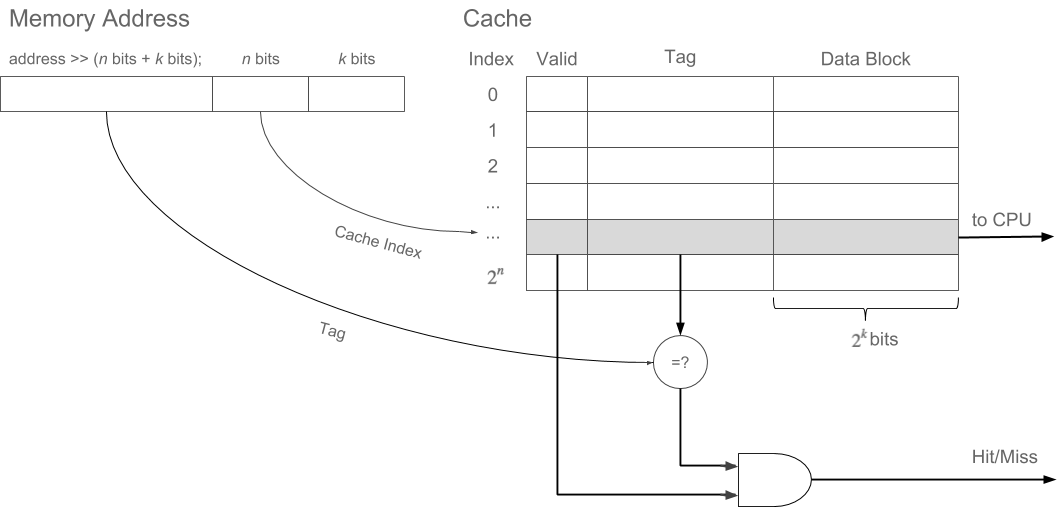
\includegraphics[width=\linewidth]{./figures/direct_cache_mapping.png}
	\caption{Direct cache address resolution.}
	\label{fig:directcache}
\end{figure}

To now locate a specific byte of data in the cache we resolve the byte address as shown in Figure \ref{fig:directcache}. Instead of performing divisions we use the least significant $k$ bits as a block offset and $n$ bits to determine the cache line index. %the Relation.. better here? *todo*

This mapping scheme causes that more than one main memory address now map to the same cache line due to the fact that the CPU cache is smaller than the main memory. Therefore, a unique identifier called \textit{tag} is introduced. The tag is defined as the remaining bits of the memory byte address. Not that $>> b$ denotes a right shift of b bits:  

\begin{small}
\begin{verbatim}
tag = address >> (nbits_ + kbits_);
\end{verbatim} 
\end{small}

%after excluding the $n$ and $k$ bits that are used for mapping, 

Tags distinguish between different memory locations that map to the same cache line. We can always match a memory address tag with the content of the mapped cache line to verify if the current block actually present in the cache line is correct for the actual memory access. Additionally a \textit{valid bit} is initialized with zero when the cache is empty and set when data is loaded into a particular cache line. This allows to determine if the information in the cache line is valid at the time of an access. 

The processor always accesses memory for instance to fetch new instructions or to load and store data in main memory while executing them. When we use this direct cache mapping, one of several situations can occur. If the mapped cache line contains invalid data, pointed out by a valid bit, the memory content needs to be loaded from main memory since the cache does not contain it. Similarly, if the cache tag fails to match the actual address tag, although it might be valid information indicated by the valid bit, the requested content needs to be loaded from main memory too, since it holds some data we are currently not looking for. In both of these two cases, requested data has to be fetched from main memory, because the cache was not able to provide the information. Either of these two cases is called a \textit{cache miss} \cite{DBLP:journals/iacr/Page02}. The other case is called a \textit{cache hit}. It is signalled when a cache line contains valid content with matching tags that is requested by the processor. In this case, the information can be gathered completely through the cache memory without resorting to the slower main memory. 

A direct-mapped cache of this scheme is very easy to compute. Indices and offsets can be computed with bit operators or simple arithmetic as showed above. Every byte address belogs in exactly one block and data gets exchanged on every cache miss. This exploits temporal locality, which assumes that older data is less likely to be requested than newer data. Basically it already is a LRU replacement algorithm. The whole concept of locality, spatial and temporal, means that the overall time needed to transfer information from one place to another is accelerated because it is likely that cache hits happen more often than cache misses. Hence, fast memory accesses exceed slower ones resulting in an overall system performance improvement. 

Altough this cache organization causes the least overhead in determining the cache line candidate, it also offers the least flexibility and may cause a lot of conflict misses \cite{DBLP:reference/db/2009}. In practice, memory blocks that belong to the same cache block are often used concurrently. Directly mapped, they always get exchanged with each other and this causes high amount data transfer and a lot of time.  

For this reason, most architectures nowadays employ \textit{set-associative caches}. This means that the cache now is divided into multiple \textit{cache sets} where each set consists of several cache lines (also called \textit{Ways}). Just like before, it depends on the memory address to which cache set the memory block is loaded in the first place. A-way set associative caches allow loading a line to A different positions. A 2-way example is illustrated in Figure \ref{fig:associativecache}. In this example, two cache lines are part of one cache set. On the one hand, it reduces the number of indices. On the other hand it increases the number of possible cache lines, where a particular memory block may be stored in the cache. 

\begin{figure*}[!ht]
	\centering
	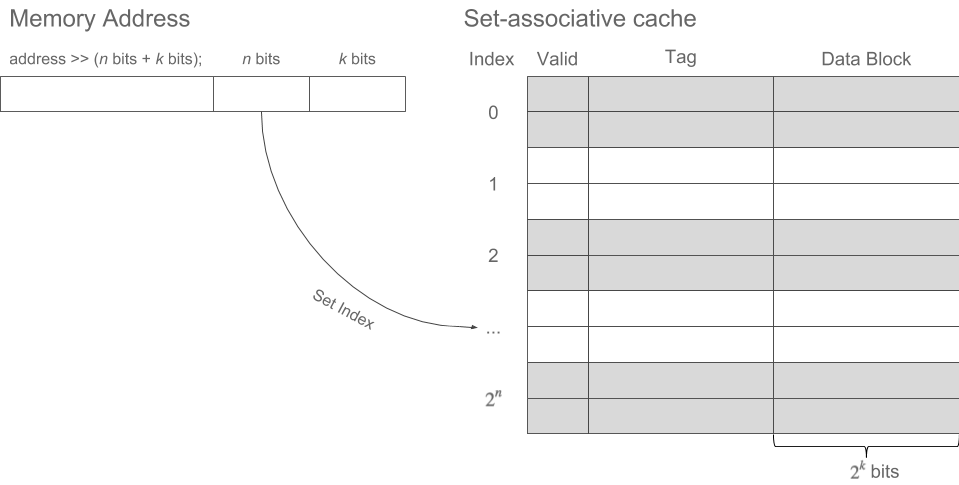
\includegraphics[scale=0.32]{./figures/a-way-set-associative.png}
	\caption{Associative cache principle.}
	\label{fig:associativecache}
\end{figure*}

Instead of forcing each memory address into one particular block, a set-associative cache permits data to be stored in any cache block that is part of the current set the address is mapped to. Following this principle there is less conflict between two or more memory addresses that map to a single cache line. One drawback of associativity is the higher effort to find valid and correct content in the cache. For every memory access, we need to compare the tag with all  the tags of A ways. 

However, this behaviour provides a lot of flexibility in terms of utilizing the principle of temporal locality. If we need to replace a cache line during a cache miss and if \mbox {A > 1}, some predetermined, smart, and most often undocumented cache replacement policy determines one from among the A candidates (e.g.: \textit{PseudoLRU} in x86 CPUs) that handles the eviction of the least recently used entry. They are much more complex and optimized compared with a simple direct-mapped LRU on how to decide which line gets evicted. If \mbox{A = 1}, the cache is called directly-mapped \cite{DBLP:reference/db/2009}.

Following the concepts of virtual memory management \cite{DBLP:books/lib/Tanenbaum09}, for data access, logical virtual memory addresses used by application code have to be translated to physical page addresses in the main memory. The \textit{Translation Lookaside Buffer} (TLB) is used as a cache for physical page addresses, holding the translation for the most recently used pages. If a virtual address is found in this cache, the translation to a physical address has no additional cost \cite{DBLP:reference/db/2009}. 

As a consequence of this virtual memory management, we need to distinguish between virtually indexed and physically indexed caches. In general, virtually indexed caches are considered to be faster than physically indexed caches \cite{DBLP:conf/uss/GrussSM15}. An advantage of virtually indexed caches is that the cache line can be looked up in parallel with the translation of the virtual address done by the TLB. However, different virtual addresses mapping to the same physical address may be cached in different cache lines in virtually indexed caches. Tags help in order to uniquely identify a specific cache line within a cache set, but even tags can either be virtually or physically. 

Summarized, caches are grouped as follows: \textit{Physically indexed, physically tagged - Virtually indexed, virtually tagged - Virtually indexed, physically tagged - Physically indexed, virtually tagged}. So this is based on wheter the index or tag correspond to virtual or physical addresses. However, within a modern computer system different types of caches are used and combined, each having advantages and disadvantages compared to each other. 

Starting with the \textit{Sandy Bridge} microarchitecture, Intel changed the mapping design for the LLC. Now the last-level cache consists of so called \textit{slices} equal to the number of CPU cores, that are connected via a ring interconnect. Each slice operates as a standard cache and has a logic portion and data array portion. The logic part handels for instance access to the data array portion and LLC misses, the data array portion stores the cache lines. "The physical addresses of data kept in the LLC data arrays are distributed among the cache slices by a hash function, such that addresses are uniformly distributed. \cite{IntelAORM2017}". In summary, to choose the slice a memory address maps to, an unpublished hash function is used which distributes addresses uniformly among all cores. Hund et al. \cite{DBLP:conf/ndss/HundWH13} and Yuval Yarom et al. \cite{DBLP:journals/iacr/YaromGLLH15} describe this hash function in more detail. 

\subsection{Page Sharing}

Operating systems and hypervisors share memory between co-operating processes to either communicate among each other, to reduce the memory footprint of a computer system by avoiding similar content in the physical memory and for TLB utilization. 

\textit{Context-aware} sharing identifies identical pages by the disk location the page contents are loaded from. In other words, shared content is loaded to physical memory just once and shared among all processes that require the use of this specific content. Therefore multiple processes can access the same physical page frame that is mapped in their virtual address space. This is known as the traditional use of shared memory. The OS similarly optimizes mapping of files, sharing text segments of executables, forking a process or using mmap \cite{DBLP:journals/corr/GrussMW15}. This form of memory sharing is implemented in all current major operating systems \cite{DBLP:journals/iacr/YaromF13}. 

Another more abrasive form is \textit{content-aware} sharing, also known as \textit{memory de-duplication}. The active physical memory is scanned continuously to identify byte-wise identical pages. These pages of possibly completely unrelated and sandboxed processes become coalesced which brings up security and privacy concerns \cite{DBLP:journals/corr/GrussMW15}. The VMware ESX \cite{DBLP:conf/osdi/Waldspurger02} hypervisor, Linux and also Windows \cite{DBLP:journals/iacr/YaromF13} \pagebreak use this technique to lower the usage of the TLB and physical memory tremendously. 

Since it is possible that non co-operating processes share physical memory, the content needs to be protected against modification. Hence, the operating system maps shared pages of this kind of \textit{copy-on-write} \cite{DBLP:books/lib/Tanenbaum09}, which prevents unrelated processes from making unauthorized write operations. While read operations are allowed, write operations cause shared pages to be copied to a separate physical memory location and to be mapped to the virtual address space of the writing process. Due to the fact that these actions cause a delay while performing the issued writing operation timing attacks become possible.  

\subsection{Cache Attacks}
\label{section:cacheattacks}

We can exploit the behaviour of CPU caches in side-channel attacks. The feasibility of cache-based side-channel attacks was already described in several publications. The first to mention the technique of cache attacks were Paul C. Kocher \cite{DBLP:conf/crypto/Kocher96}, John Kelsey et al. \cite{DBLP:conf/esorics/KelseySWH98 } and later on Page \cite{DBLP:journals/iacr/Page02}. Basically, not the mathematical properties of an algorithm are attacked, but rather an adversary tries to collect enough side-channel information leaked from the implementation of a cryptographic function for cryptanalysis. With enough side-channel information, breaking a cipher gets trivial. In the past few years, several attacker models, which we now describe, derived and have been investigated quite extensively. Today cache-based side-channel attacks can be divided into three main categories. 

\textit{Time-driven} attacks exploit the execution time of an algorithm which depends on its cache access pattern. Bernstein described a cache-timing attack on an AES implementation were he was able to recover the secret key \cite{misc:bernstein2005}. 

In \textit{Trace-driven} attacks \cite{DBLP:journals/iacr/GallaisKT10, DBLP:conf/icics/AciicmezK06} additional detailed execution  side-channel information such as registered power consumption or electromagnetic emanations are required. They are a particular threat to embedded devices since the attacker often needs to have physical access to the device, in opposite to desktop and server implementations, that are mostly targets of access- and time-driven cache-attacks. 

\pagebreak
In \textit{access-driven} attacks, the adversary learns which cache lines are accessed during the execution time of an algorithm. Generally, they are categorized as follows: \textit{Flush+Reload} \cite{DBLP:journals/iacr/YaromF13} and \textit{Prime+Probe} \cite{DBLP:journals/iacr/OsvikST05, DBLP:journals/joc/TromerOS10}. 

Flush+Reload is an improvement of an attack proposed by Gullash et al. \cite{DBLP:journals/iacr/BangerterGK10} and attacks the L3 cache while the original attack targets the L1 cache. Both attacks rely on the availability of shared memory. A newer attack called \textit{Flush+Flush} \cite{DBLP:journals/corr/GrussMW15} which pretends to be a faster and stealthier alternative to previous access-driven attacks with fewer side effects on the cache, appeared recently. Basically, they exploit the cache as a source for side-channel information by using the knowledge of cache mechanisms like the replacement algorithm, eviction of cache lines, the inclusively of caches, and the mapping itself. In these attacks, the CPU cache leaks infomration about memory accesses to an adversary, who is able to monitor cache hits and misses. Attackers then make use of the gathered hit/miss information to recover cryptographic keys. 

Some attacks rely on the availability of shared memory, while it is not a working condition for others. If two processes physically share main memory, an attacker starts by flushing the cache before being halted and scheduled out by the CPU. After regaining control, the process is able to monitor cache hits and misses by measuring the latency. With this information, memory accesses of the other process can be reproduced. With todays shared L3 (LLC) cache among the cores, it is not even necessary to interrupt the victim process. Both processes can run on different cores and work on the same L3 cache. Constantly flushing a single cache line and reloading is the underlying concept of Flush+Reload. Possible targets are often shared libraries (e.g.: \textit{OpenSSL}), as they in practice reside at a single physical place in memory only and therefore are mapped into the virtual memory space of every process that uses it. 

Without having physically shared memory, knowledge about the replacement strategy is being used. Since we know how cache sets work, the attacker process can initialize the cache with some data knowing that a number of \textit{A} memory accesses are needed to fill an entire cache set. When \textit{A} different addresses have occured, the cache logic needs to evict cache lines using the underlying cache replacement algorithm. After waiting for the victim process to access memory locations and therefore changin the cache data using the replacment algorithm, the attacker again accesses the data and notes which data has been evicted. This technique allows to gain information about the memory accesses of the victim and is used by the Prime+Probe attack. 

\subsection{QEMU}
\label{section:qemuinternals}

The \textit{Quick Emulator} or for short \textit{QEMU} is a machine emulator to run an unmodified target operating system with all its applications in a virtual machine. It emulates many different architectures (e.g.: X86, ARM, SPARC) and runs on several architectures. Basically, an emulated CPU executes target instructions. However, the reason for its flexibility and speed is the implementation of a so-called \textit{dynamic translator}. It performs a runtime conversion of a target CPU instruction to the host instruction set, producing a binary which is stored in a \textit{translation cache} (TC) for later use. The advantage compared to a conventional interpreter is that target instructions are fetched and decoded only once \cite{DBLP:conf/usenix/Bellard05}. 

\subsubsection{Dynamic binary translation}

This dynamic binary translation (DBT) reduces overhead and is the reason of fast simulation speed. It devides target binary code into chunks of code called \textit{basic blocks} (BBs). Starting, when the program counter of an emulated system points to a BB the first time, QEMU translates this chunck of target code to host code up to the next jump or instruction using the \textit{tiny code generator} (TCG) front end. These translated pieces are called \textit{translated blocks} (TBs). Afterwards this intermediate code is cached in the TC and if needed translated to a host instruction by the TCG back end before execution. The TC provides a noticeable speedup allowing to skip the TCG translation process, which is the most expensive part during the execution loop. It is accessed repeatedly by the host CPU. This process is described in Figure \ref{fig:qemusim}.

\begin{figure}[!ht]
	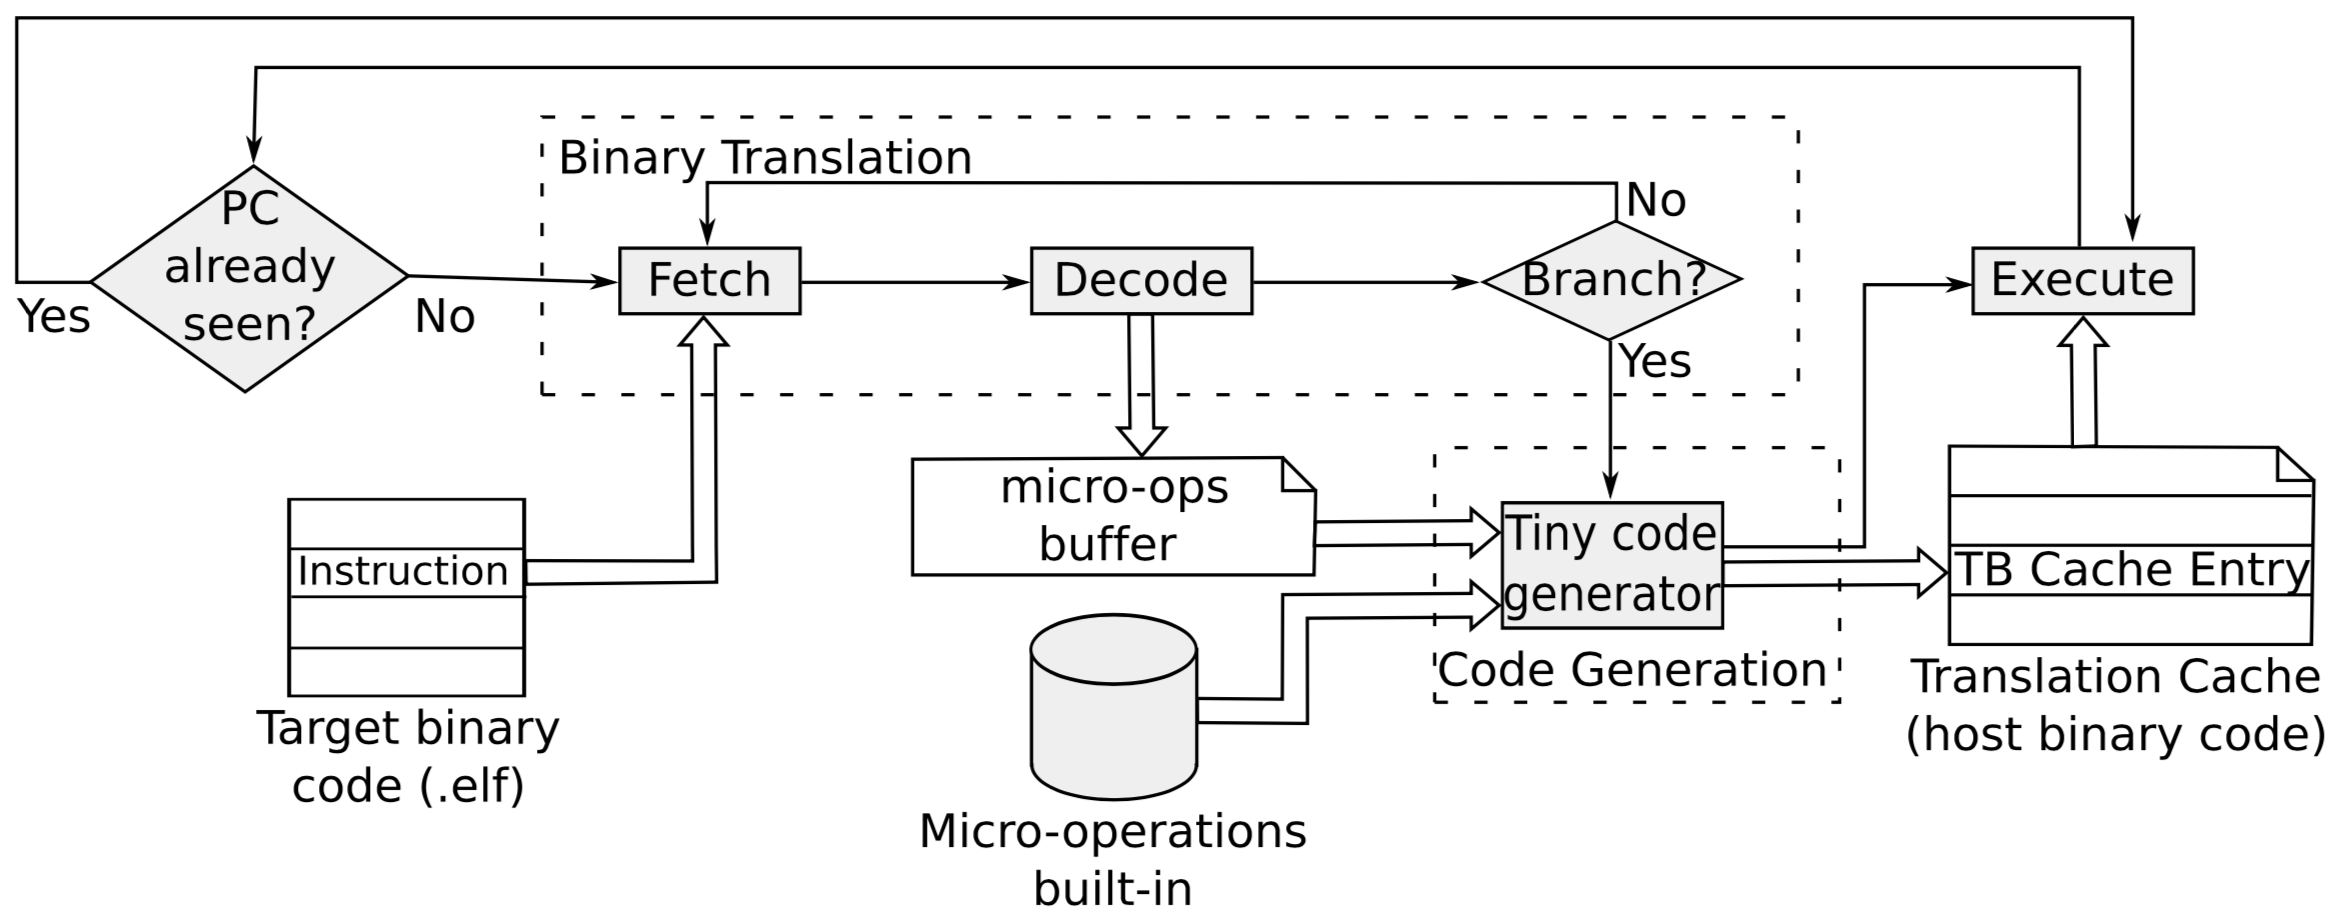
\includegraphics[width=\linewidth]{./figures/QEMU_simulation_model.png}
	\caption{QEMU simulation model \cite{DBLP:conf/codes/GligorFP09}.}
	\label{fig:qemusim}
\end{figure}

\subsubsection{Memory Emulation}

QEMU supports a \textit{software MMU} in order to be able to launch any OS. In software MMU mode, QEMU uses a TLB which is quite similar to the traditional hardware TLB idea. To speed up the translation process from a guest virtual address to a host virtual address, the TLB therefore stores an offset. 
\begin{small}
\begin{spverbatim}
	haddr = addr + 
	env->tlb_table[mmu_idx][index].addend;
	
\end{spverbatim}
\end{small}


This MMU translation is done at every memory access \cite{DBLP:conf/usenix/Bellard05}. It searches this TLB table first and fills the offset into the table on a miss, done by a macro function. Additionally, besides speeding up the translation from guest virtual addresses to host virtual addresses, this model can speed up the process of dispatching I/O emulation functions according to guest virtual address too \cite{DBLP:conf/dasc/DungTT14}. 

\section{Methodology}

\subsection{Cache model}
\label{subsection:cachemodel}

The goal is to implement a flexible cache model whose characteristics are easily adjustable, to be able to simulate different cache models that match a wide range of actual or future CPU cache models. Therefore, three main characteristics need to be adjustable: Cache capacity, block size and associativity. However, todays CPU caches do not simply cache chunks of memory when it is accessed by a load or store operation. Data can be speculatively loaded to the L1 DCACHE using software prefetching, hardware prefetching, or any combination of the two \cite{IntelAORM2017}. These speculative fetching algorithms mostly rely on upublished mechanisms and cannot be considered in the scope of this work. Nevertheless, regarding the cache associativity we need to distinguish between direct and associative mapped caches. 

For direct mapped caches, the relation 
\\
$cache\ capacity\ /\ cache\ block\ size$ 
\\
returns the amount of cache lines needed for this particular combination of cache capacity and block size. To calculate the number of bits needed for the block offset as well as cache index, we use the definition of the logarithm: $x = log_a (y) \equiv y = a^x$. To be able to map every cache line we caclulate the number of $n$ bits with $log(cache\ lines) / log(2)$ and to address each and every byte in a cache line we use $log(block\ size) / log(2)$ for the  calculation of $k$ bits. 

For associative mapped caches, the amount of cache sets needed with any selected cache configuration results from 
\\
$(cache\ capacity\ /\ cache\ block\ size)\ /\ association$. 

The number of $n$ bits can now be calculated with $log(cache\ size) / ways) / log(2)$. Clearly, the calculation of the block offset happens in exactly the same way as for direct mapped caches. Moreover, the number of different cache lines in a cache set is equal to the association. Note that our cache model does not support the mapping design for LLC slices that started with the Sandy Bridge microarchitecture recently \label{section:cachemapping}. See Listing \ref{lst:memcache} below.

\begin{small}
\begin{lstlisting}[caption={Basic cache structure.},label={lst:memcache}, captionpos=b, language=C]
struct MemCache {
uint32_t size_;
uint32_t ways_;
uint32_t kbits_;
uint32_t nbits_;
uint32_t lines_;
uint32_t sets_;
uint32_t block_size_;
CacheLine *cache_line_ptr_;
CacheSet *cache_set_ptr_;
uint64_t cache_hits_;
uint64_t cache_misses_;
uint64_t replacements_;
};
\end{lstlisting}
\end{small}

In a nutshell, the implemented \textit{cache controller} has the following capabilities: 
%\begin{small}
\begin{itemize}
	\item The creation of a custom configurable cache.
	\item Calculation and initialization of all necessary values depending on configurated mapping type (direct / associative).
	\item Memory allocation and free of all required structures.
	\item Logic to resolve any (physical or virtual) given memory address and produce cache hits and misses.
	\item Perform arbitrary amount of real-time latency on cache misses. 
	\item Various posibilities to monitor and compare cache behaviour. 
	\item Complete cache flush.
\end{itemize}
%\end{small}


In oder to be able to support both types of cache mappings, the controller distinguishes between the chosen mapping and allocates either the amount of calculated cache lines without using an associative set structure underneath, or it automatically groups cache lines into a number of therefore calculated set structures. See Listing \ref{lst:linessets} below. 

\begin{small}
\begin{lstlisting}[caption={Operational cache  structures.},label={lst:linessets}, captionpos=b, language=C]
struct CacheSet {
uint32_t set_lines_;
CacheLine *set_line_ptr_;
};

struct CacheLine {
bool valid_;
size_t tag_;
uint8_t line_data_[CACHE_BLOCK_SIZE];
};
\end{lstlisting}
\end{small}


With this structure, finding the corresponding cache line or cache set can simply be computed using bit operators. Remember, the index that relates to our line/set can be determined by the number of $nbits\_$. A right shift on the given memory address $>> kbits\_$ and left shift $<< tag\_bits\_$ finally gives us our index. By simply adding the index to our cache line/set pointer, illustrated in Listing \ref{lst:detindex}, we can quickly determine the corresponding operational structure.  

\begin{small}
\begin{lstlisting}[caption={Determining the set  index.},label={lst:detindex}, captionpos=b, language=C]

set_index = (((addr >> cache->kbits_) 
<< (sizeof(addr) * 8 - cache->nbits_))
>> (sizeof(addr) * 8 - cache->nbits_));

CacheSet *cache_set = 
cache->cache_set_ptr_ + set_index;

\end{lstlisting}
\end{small}


\begin{figure*}[!ht]
	\centering
	\begin{small}
	\begin{lstlisting}[caption={Allocation of memory region for system memory.},label={lst:allocsysmem}, captionpos=b, language=C]

	void memory_region_init_rw_mod(MemoryRegion *mr, Object *owner, 
	const char *name, uint64_t ram_size, Error **error_fatal) {
	
	memory_region_init(mr, owner, name, ram_size);
	mr->ram = true;
	mr->ram_device = true;
	mr->ops = &ram_mem_ops;
	mr->opaque = mr;
	mr->terminates = true;
	mr->destructor = mem_destructor_ram;
	mr->dirty_log_mask = tcg_enabled() ? (1 << DIRTY_MEMORY_CODE) : 0;
	mr->ram_block = qemu_ram_alloc(ram_size, mr, error_fatal);
	};

\end{lstlisting}
	\end{small}

\end{figure*}

Depending on the operational structure one of two situations occur. If we directly point at our cache line we simply have to check if the content in this particular cache line is valid and correct by checking the valid bit and comparing the tag also acquired from the given memory address. If we point at a cache set, every cache line of the A-ways need to be checked \ref{section:cachemapping}. Finally the usage of replacement algorithms becomes as easy as adding structure members and develop a corresponding logic that can be used by this check function. To generate a simulation as accurate as possible either simple LRU as well as a random replacement algorithm where implemented. In contrast to the least recently used principle the random algorithm tries to uniformly distribute the chosen cache lines that gets evicted. 

\subsection{On-line simulation using QEMU}

The basic idea is to use this generic, open source machine \& userspace emulator and virtualizer to establish a working on-line LLC cache simulation. This should result in mentionable advantages over known simulations. An example of a cache simulation was integrated to the \textit{Transaction Level Modeling} (TML) simulator using ARM architecture by Ardavan Pedram et al. \cite{DBLP:conf/iess/PedramCG09}. They archieved good results in terms of accuracy simulating miss rates. However, an implementation in QEMU would give a fair speed advantage over TML, as well as easy to adapt simulation of different simulation architectures. Tran Van Dung et al. \cite{DBLP:conf/dasc/DungTT14} implemented a cache simulation using QEMU helper functions and modifications in the process of translating the guest virtual address to host virtual address or dispatching guest virtual address to I/O emulation functions. Their cache simulator is called using virtual program counters and we are not sure about the mapping or the cache model in the background. Nevertheless, they seem to archive miss/hit rates but no actual cache attack was proven in that article. Also Valgrind \cite{valgrindusrman} can be used for cache evaluation. It can output cahe miss and hit rates, but it does not account TLB misses or kernel process activity. 

Using and modifying QEMU's source code benefits in full control over virtualized hardware, which means it should be possible to adapt the execution process, record and redirect all main memory accesses. Specific embedded devices can be simulated adding machine descriptions and new emulated devices to the source code. A good example implementation can be found within the ARM xilinx-zynq target \cite{zynq2017}. When emulating a \textit{X86-64bit} or \textit{X86-32bit} system, naturally different header files are used in contrast to emulate ARM or SPARC architecture. Since we target a cache simulation of current Intel processors the header file of our importance names \textit{QEMU PC System Emulator} and can be found in \textit{pc.c}. We adapted the process of creating our emulated system and therefore started with modifying the allocation of main memory on our desired target \textit{i368} to gain control over type and features of our main memory. Listing \ref{lst:allocsysmem} shows the creation of our memory region we use for the systems main memory. This function replaces the original memory allocation while creating the actual system. 

In general, the function \textit{memory\_region\_allocate\_system\_memory()} allocates the system main memory for every platform we know of. Furthermore, this function is useful to allocate and initialize the cache environment (see Listing \ref{lst:memcache}) in an early phase of the system creation too. 

The whole code path is as following:
 
 \begin{small}
\begin{spverbatim}
	pc_init1() -> pc_memory_init() -> memory_region_allocate_system_memory() -> allocate_system_memory_nonnuma() -> memory_region_init_rw_mod()
	
\end{spverbatim}
 \end{small}

We defined so-called \textit{memory-ops} for our newly created ram device (short for random-access memory device). From our understanding of their implementation in QEMU at this time, memory-ops are called everytime the CPU needs to fetch any content from this device with its physical guest address. We tried to utilize these functions by calling the check function of cache model described in \ref{subsection:cachemodel}. Our goal was to simulate L3 access-driven side-channel attacks and this conception theoretically fits a L3 cache simulation, which is physically indexed in most CPU architectures due to several reasons. 


\begin{figure*}[!h]
	%\centering
	\begin{small}
		\begin{lstlisting}[caption={Calculation and usage of physical address on TLB translation.},label={lst:physcalulationsoftmmu}, captionpos=b, language=C]
		
uintptr_t guest_phys_haddr;
guest_phys_haddr = addr - env->tlb_table[mmu_idx][page_index].ADDR_READ + 
	env->tlb_table[mmu_idx][page_index].phys;

if(cache_simulation_active()){
	check_hit_miss(guest_phys_haddr, 0);
}

uintptr_t hostaddr = addr + env->tlb_table[mmu_idx][page_index].addend;

res = glue(glue(ld, USUFFIX), _p)((uint8_t *)hostaddr);
		
		\end{lstlisting}
	\end{small}
\end{figure*}


\subsubsection{Experiments}

Basically, we tried to experiment conceptionally equal as doing it on real hardware. To speed up the boot process (we used a \textit{minimal Ubuntu distribution}), a QEMU monitor command \cite{wiki:QEMUmonitor} namely \textit{cache\_enable} was implemented, that allows to boot the kernel without the excessive use of the cache model during the booting phase. With a fully functional operating system we used a repository that contains several tools to perform Flush+Flush and related attacks \cite{misc:flushflush2016}, that all target the LLC. 

A simple calibration tool measures time differences of cache hits and cache misses and even provides a certain threshold for the actual attack beforehand, by using the \textit{rdtsc} instruction that produces subnanosecond resolution timestamps. These timestamps have been proven to be correct regarding its underlaying rdtsc implementation in QEMU. They actually just differ from the corresponding host system timestamp by a given offset, so generally rdtsc should work the same way in this emulation as it does on real hardware. Additionally, these tools make use of the \textit{clflush} instruction which is not implemented in QEMU and originally produces non operational intermediate code. Therefore, we defined a helper function (described by e.g.: Tran Van Dung et al. \cite{DBLP:conf/dasc/DungTT14}) and inject a function call to the translated block that is stored in TC. Our function call performes a simple flushing operation of all cache lines. With this modification we can ensure to always wipe our cache when a user program issues a clflush instruction.  

Nevertheless, the produced \textit{hit-histogram} should distinguish from the \textit{miss-histogram} in a way, that the peak of nearly equally distributed access times produced by cache hits and the access times of cache misses must be clearly shifted on the x-axis. Otherwise cache misses and cache hits are not recognizable and monitorable which an adversary must be capable of to perform an actual attack \ref{section:cacheattacks}. 

\begin{figure*}[!ht]
	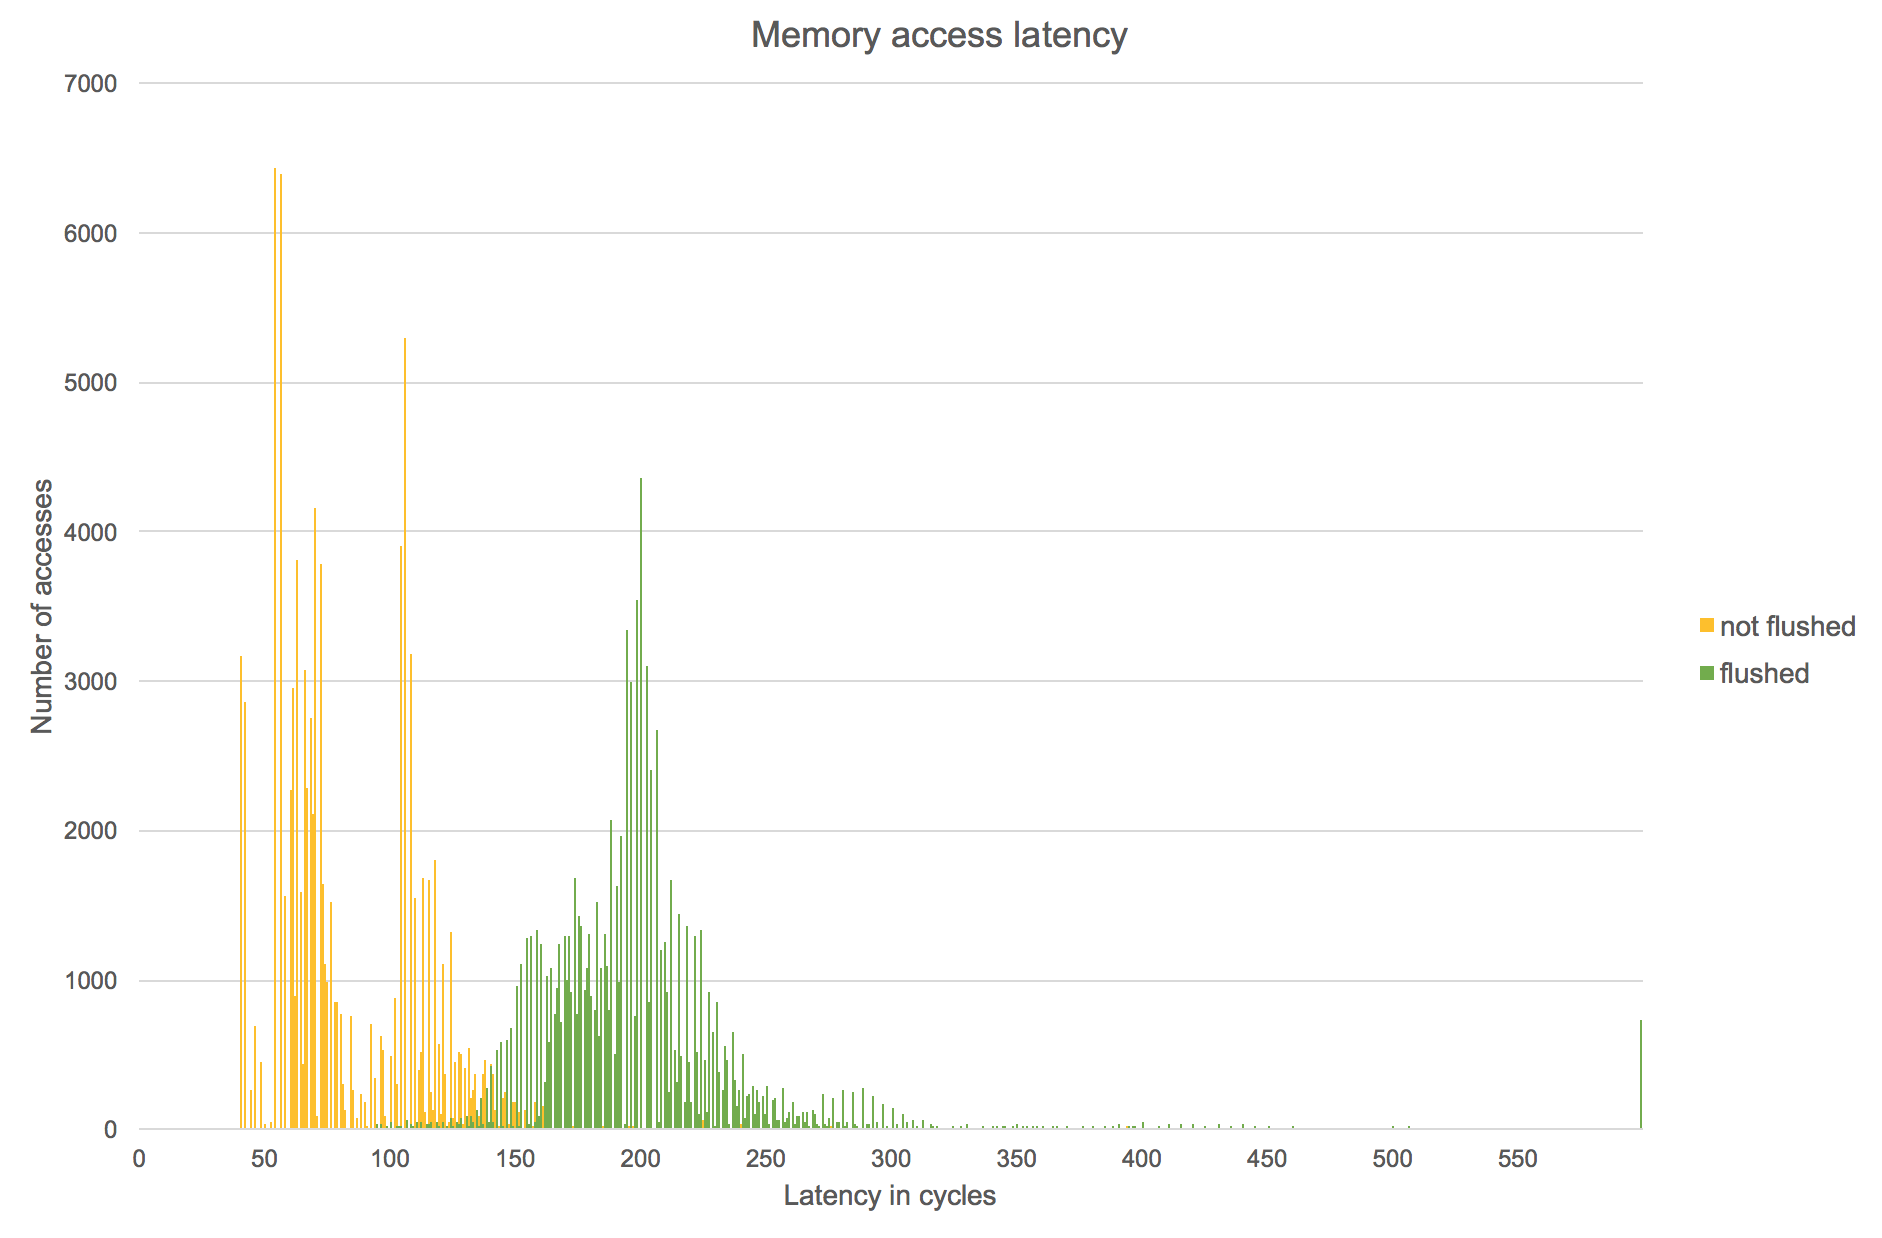
\includegraphics[width=\linewidth]{./figures/hist.png}
	\caption{Histogram of associative cache simulation.}
	\label{fig:hist}
\end{figure*}

Since all our efforts failed to get usefull timing data out of our simulation, we discovered that MMU faults caused by accessing our I/O device apparently trigger memory-ops but not subsequent accesses. In fact, we assume that needed instructions triggered by a user program are fetched only once, translated via the QEMU internal translation process (tiny code generator \ref{section:qemuinternals}) and then called from the TC without calling the memory-ops anymore which absolutely is essential for access-driven side-channel attacks. 

To aquire traces of memory accesses, issued by user programs that are already translated, we tried to modify the instruction execution process to that effect. When fetching code from guest memory, the MMU translation from guest virtual address to host virtual address is done at every memory access, theoretically. Therefore we had to modify the behaviour of the softmmu. After excessive debugging we found promising pieces of code that became candidates for modification right at the point where a CPU load or CPU store operation tries to aquire the offset from the TLB. Remember, the TLB implementation in QEMU translates virtual guest to virtual host addresses \ref{section:qemuinternals} which both are unsufficient for our needs, simulating a LLC. We had to calculate the guest physical address and managed to do so by adding an additional member called \textit{phys} to the \mbox{\textit{CPUTLBEntry}} structure to store an offset to calculate the physical guest address. From now on, we add the calculation of the physical guest address given a virtual guest address everytime the softmmu performs its obligatory translation via our modified TLB table entry. This physical guest address can then be used for cache simulation. Alongside those translations found in \textit{softmmu\_template.h} we found generic load/store macros in \textit{cpu\_ldst\_template.h} which we modified as well. Listing \ref{lst:physcalulationsoftmmu} shows an example of this calculation.   

\begin{lstlisting}[caption={Memory access performed by user program \cite{misc:flushflush2016}.},label={lst:maccess}, captionpos=b, language=C]

void maccess(void* p){
asm volatile ("movq (%0), %%rax\n"
:
: "c" (p)
: "rax");
};

\end{lstlisting}

Although we archieved better resolution on the histograms now, we where not able to completely account for all user memory accesses. Still, accesses of the form showed in \mbox{Listing \ref{lst:maccess}}, are not recognized by our cache simulation right now. Finally, Figure \ref{fig:hist} shows the best calibration histogram we got, simulating an associative cache with a capacity of 128 KiB and block size of 64 byte.  

\subsubsection{Conclusion}

The best resolution we were able to archieve still is not sufficient enough to simulate access-driven cache attacks. One assumption is that QEMU's internal TCG optimizes the process of executing CPU load and store instructions on user programs in some way we can not completely understand right now. We managed to raise the resolution from the first naive approach using mem ops, considerably by instrumenting the TLB at the end. A repository of this work can be found here \cite{misc:qemusim2017}.

\subsection{Off-line simulation}
\label{section:offlinesim}

In this section we use our cache model as a standalone software instrumenting memory trace files to simulate the difference between various cache configurations in terms of capacity, block size and associativity. We added a main function to control and track our cache simulation. Therefore, we use the programming language \textit{C++} because its libraries help to facilitate the statistical evaluation. The cache model itself still is classic \textit{C} but we extended its functionality to improve the overall simulation. This process is now described briefly. 

Repeated cache misses have tremendous impact on the performance of a CPU. Imagine the CPU needs to load data 100 times in a row and perfectly hits the L1 cache with a latency of 1ns for all those load instructions. This is called 100\% hit rate and results in 100 nanoseconds fetching time alltogether. Now, assume the hit rate of the cache drops just for 2\%. That means out of 100 loads 98 of them still have a latency of 1ns but two of them hit the higher L2 cache with a latency of 10ns. This two percent reduction in hit rate has an impact of nearly 20 percent on the performance of the CPU. Naturally, it gets worse when needed data must be fetched from main memory with a latency of about 60-120ns. A difference of 2\% in L1 hit rate can then nearly double the total time the CPU needs to execute the code. 

As a consequence CPU manufacturer use different techniques of data prefetching in modern microprocessors nowadays \cite{IntelAORM2017} to have data in the lowest level possible when it is needed. This can not be simulated decently but, the advantages of using a cache hierarchy can be proven by calculating the \mbox{\textit{Average Access Time}} (AAT). The AAT depends on the miss rate of all the structures that it searches through for the data \cite{DBLP:books/daglib/0028244}. When the memory hierarchy conceptionally only consits of L1 cache and main memory, the average access time can be calculated with: 
\\\\
$hit\ time_{c} + (miss\ rate_{c} * miss\ penalty_{m})$ 
\\

Where \textit{c} stands for \textit{cache} and \textit{m} for \textit{main memory}. The values that are used for the following calculations are shown in Table \ref{table:AAT}. This example shows on how to take all cache levels into account: 

\begin{table}
	\begin{tabular}{|c|c|c|}
		\hline
		Level & Hit Latency (ns)   & Miss Rate\\ [0.5ex] 
		\hline\hline
		L1 cache 		   & 1 							& 5\% 				\\ 
		L2 cache 		  & 4							& 1\% 				\\ 
		L3 cache 		  & 10 							& 0,2\% 		   \\ 
		Main Memory   & 80 							& 0\% 			    \\
		\hline
	\end{tabular}
\caption{Memory hierarchy example of hit latency and miss rates.}
\label{table:AAT}
\end{table}

ATT = L1 cache + L2 cache + L3 cache + main memory) = $1 + (0.05 * (4 + 0.01 * (10 + 0.002 * 80))) = 1.20508ns$. Hence, the time to fetch data from any cache is much less than the hit time for the main memory. This obviously improves the AAT significantly. In order to show the difference we now assume to only have a cache hierarchy of one cache, thus L1 cache + main memory, and get: $1 + (0.05 * 80) = 5ns$. Basically we see that the advantage of having two additional higher cache levels loweres the average access time about 76\%. The cache simulation supports up to three different cache levels by using the AAT. Therefore, latency and miss rates are freely adjustable.  

\subsubsection{Experiments}

To simulate different cache configurations we generated trace files using \textit{Pin}, different libraries (e.g.: openSSL) and compressing software. Pin is a platform for creating analysis tools. A pin tool performes instrumentation by taking control of a program just after it loads into the main memory. Instrumentation is performed at run time on the compiled binary file, thus no recompiling is needed. In general, it allows context information such as memory accesses to be passed to injected code \cite{IntelPin}. 

We generated several memory trace files using the pin platform. In fact, we encrypt 35.919.013 bytes of data using \textit{AES} with \textit{cipher block chaining (CBC)} mode of operation, the stream cipher \textit{ARC4} and the elliptic curve encryption \textit{SECP256k1} used in bitcoin. Furthermore, we generated a memory trace called \textit{tar\_unzip} whe we unzip the same size of data used in previous memory traces. However, we now deal with virtual memory addresses and therefore simulate a L1 data cache with two higher cache levels before data is fetched from main memory. 

First, we want to experiment with different cache characteristics such as cache capacity, block size, associativity and also cache mapping. Therefore we use fixed values for cache access times and miss rates on higher cache levels in order to concentrate on different cache specifications only. We again use the values from Table \ref{table:AAT} for all simulations. You have to consider that the miss rate of the L1 cache now is determined by the cache simulation itself. Different cache characteristics show different miss rates depending on how the actual cache model fits the current operation and therefore the data that needs to be fetched by the CPU.

\begin{figure}[!ht]
	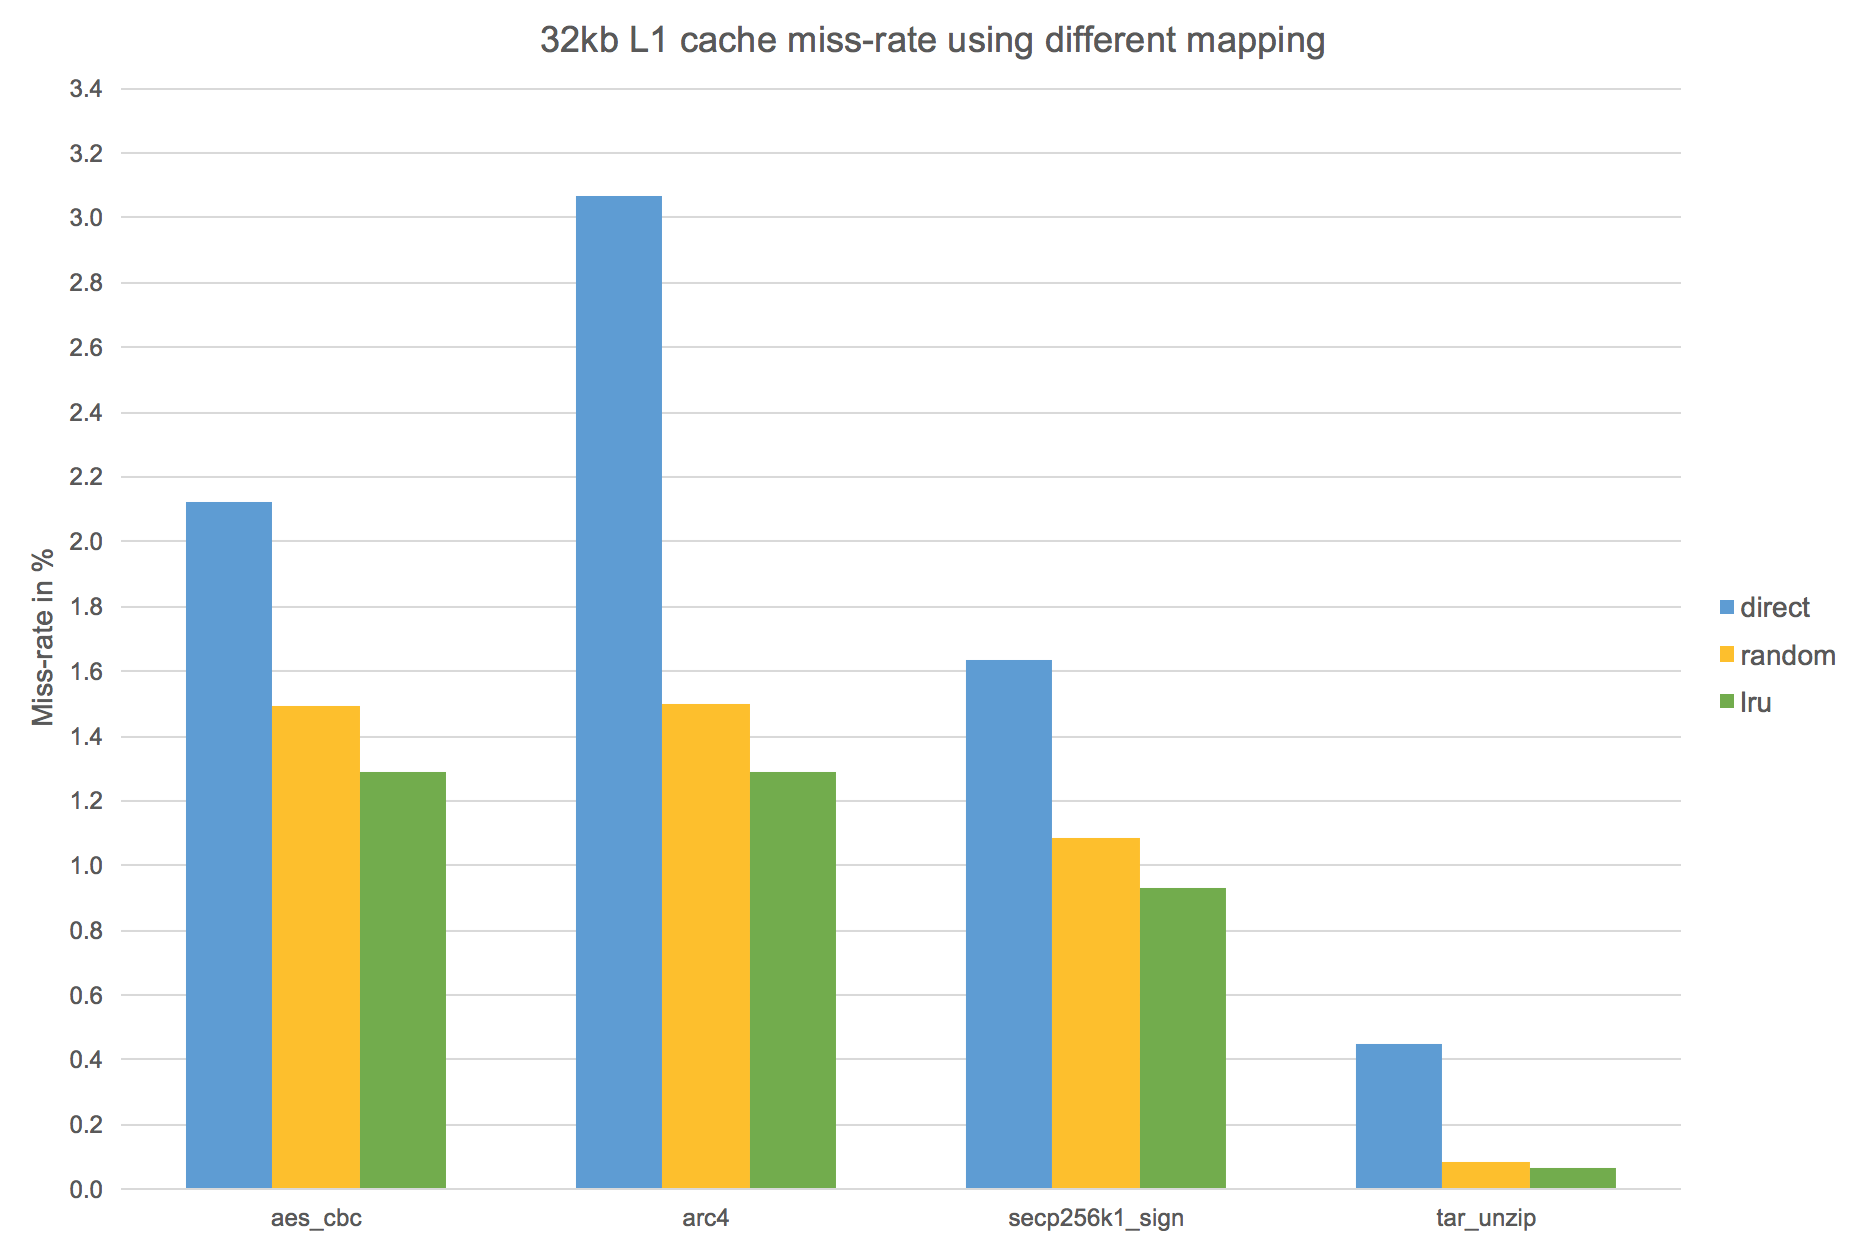
\includegraphics[width=\linewidth]{./figures/chart_diff_mapping_bar.png}
	\caption{Illustrating cache miss-rate with different cache mapping.}
	\label{fig:diff_mapping}
\end{figure}

\begin{figure*}[!ht]
	\centering
	\begin{minipage}{.5\textwidth}
		\centering
		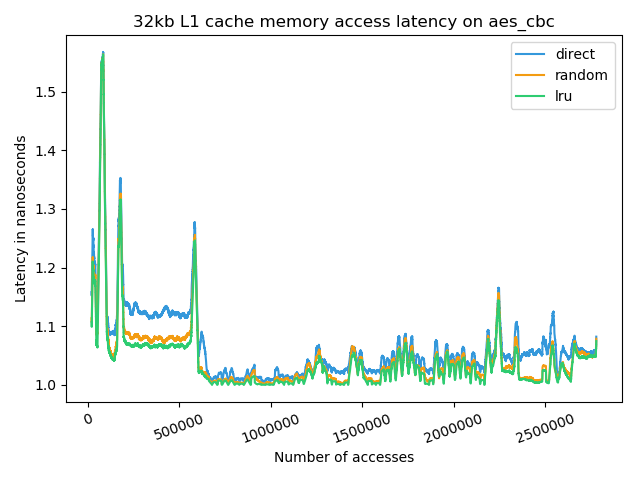
\includegraphics[width=\linewidth]{./figures/15-04-2018_15-02-49_aes_cbc-line_fetch_ns_rwindow=20000.png}
		\caption{Cache mapping comparison on AES.}
		\label{fig:diff_mapping_aes}
	\end{minipage}%
	\begin{minipage}{.5\textwidth}
		\centering
		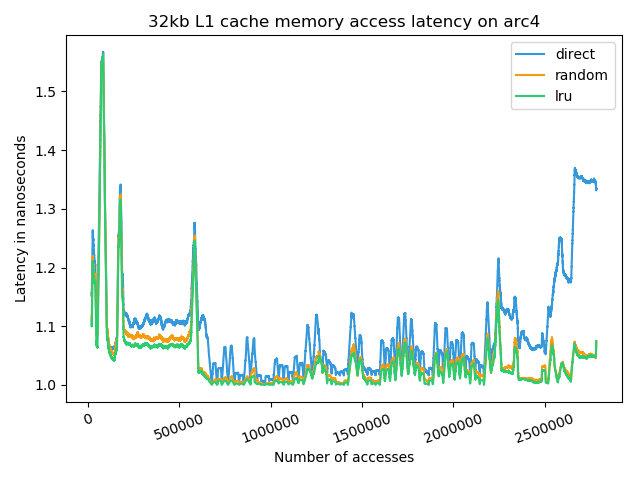
\includegraphics[width=\linewidth]{./figures/15-04-2018_15-05-24_arc4-line_fetch_ns_rwindow=20000.png}
		\caption{Cache mapping comparison on ARC4.}
		\label{fig:diff_mapping_arc4}
	\end{minipage}
\end{figure*}

\begin{figure}[!ht]
	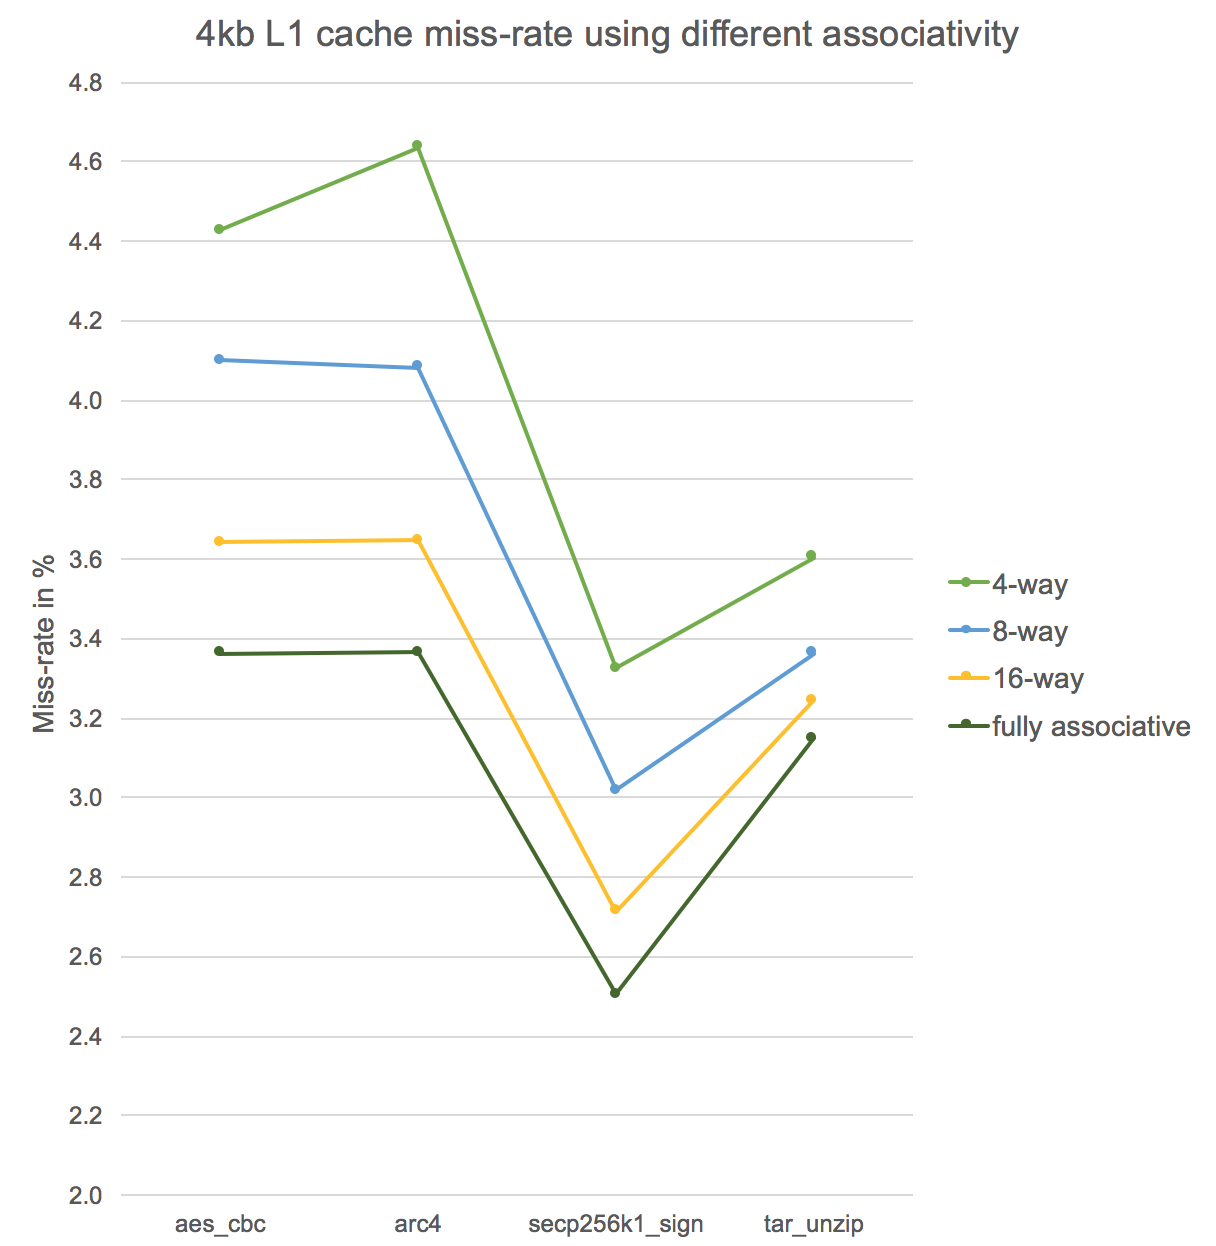
\includegraphics[width=\linewidth]{./figures/chart_diff_ass_line.png}
	\caption{Comparison of different associativity.}
	\label{fig:fully_associative}
\end{figure}

Different cache mapping, is it either a direct mapped cache or an set associative cache, clearly can make a big difference in cache performance. And so does the replacement algorithm when we are talking about associative caches. The associative mapping scheme is the most widely used today, because the prooved to have a good overall performance. In addition, a more complex replacment algorithm can result in supplementary performance gains. 

Figure \ref{fig:diff_mapping} shows a comparison between one direct and two set associative caches throughout all test cases. Two different replacement algorithms uniquely characterize each set associative cache. We used a cache capacity of 32 KiB, a block size of 64 byte and a 8-way associativity for associative caches. Due to the fact that associativity generally produces less conflicts between two or more memory addresses that map to a single cache line \ref{section:cachemapping}, we observe that both set associative caches can easily outperform its opponent. On \textit{aes\_cbc} we see the biggest advantage of associativity in the first quater of memory accesses. Obviously, the smarter replacement algorithm, has advantages in this phase compared to a simple random algorithm. The LRU algorithm better optimizes the eviction of cache lines in terms of the temporal locality principle \ref{section:cachemapping}. This is illustrated in Figure \ref{fig:diff_mapping_aes}. An interesting test case happens to be \textit{arc4}. Since the direct cache mapping performs worse all the way, it even produces a lot of cache line conflicts at the end of the process. Therefore see Figure \ref{fig:diff_mapping_arc4}.

 \begin{figure*}[!ht]
	\centering
	\begin{minipage}{.5\textwidth}
		\centering
		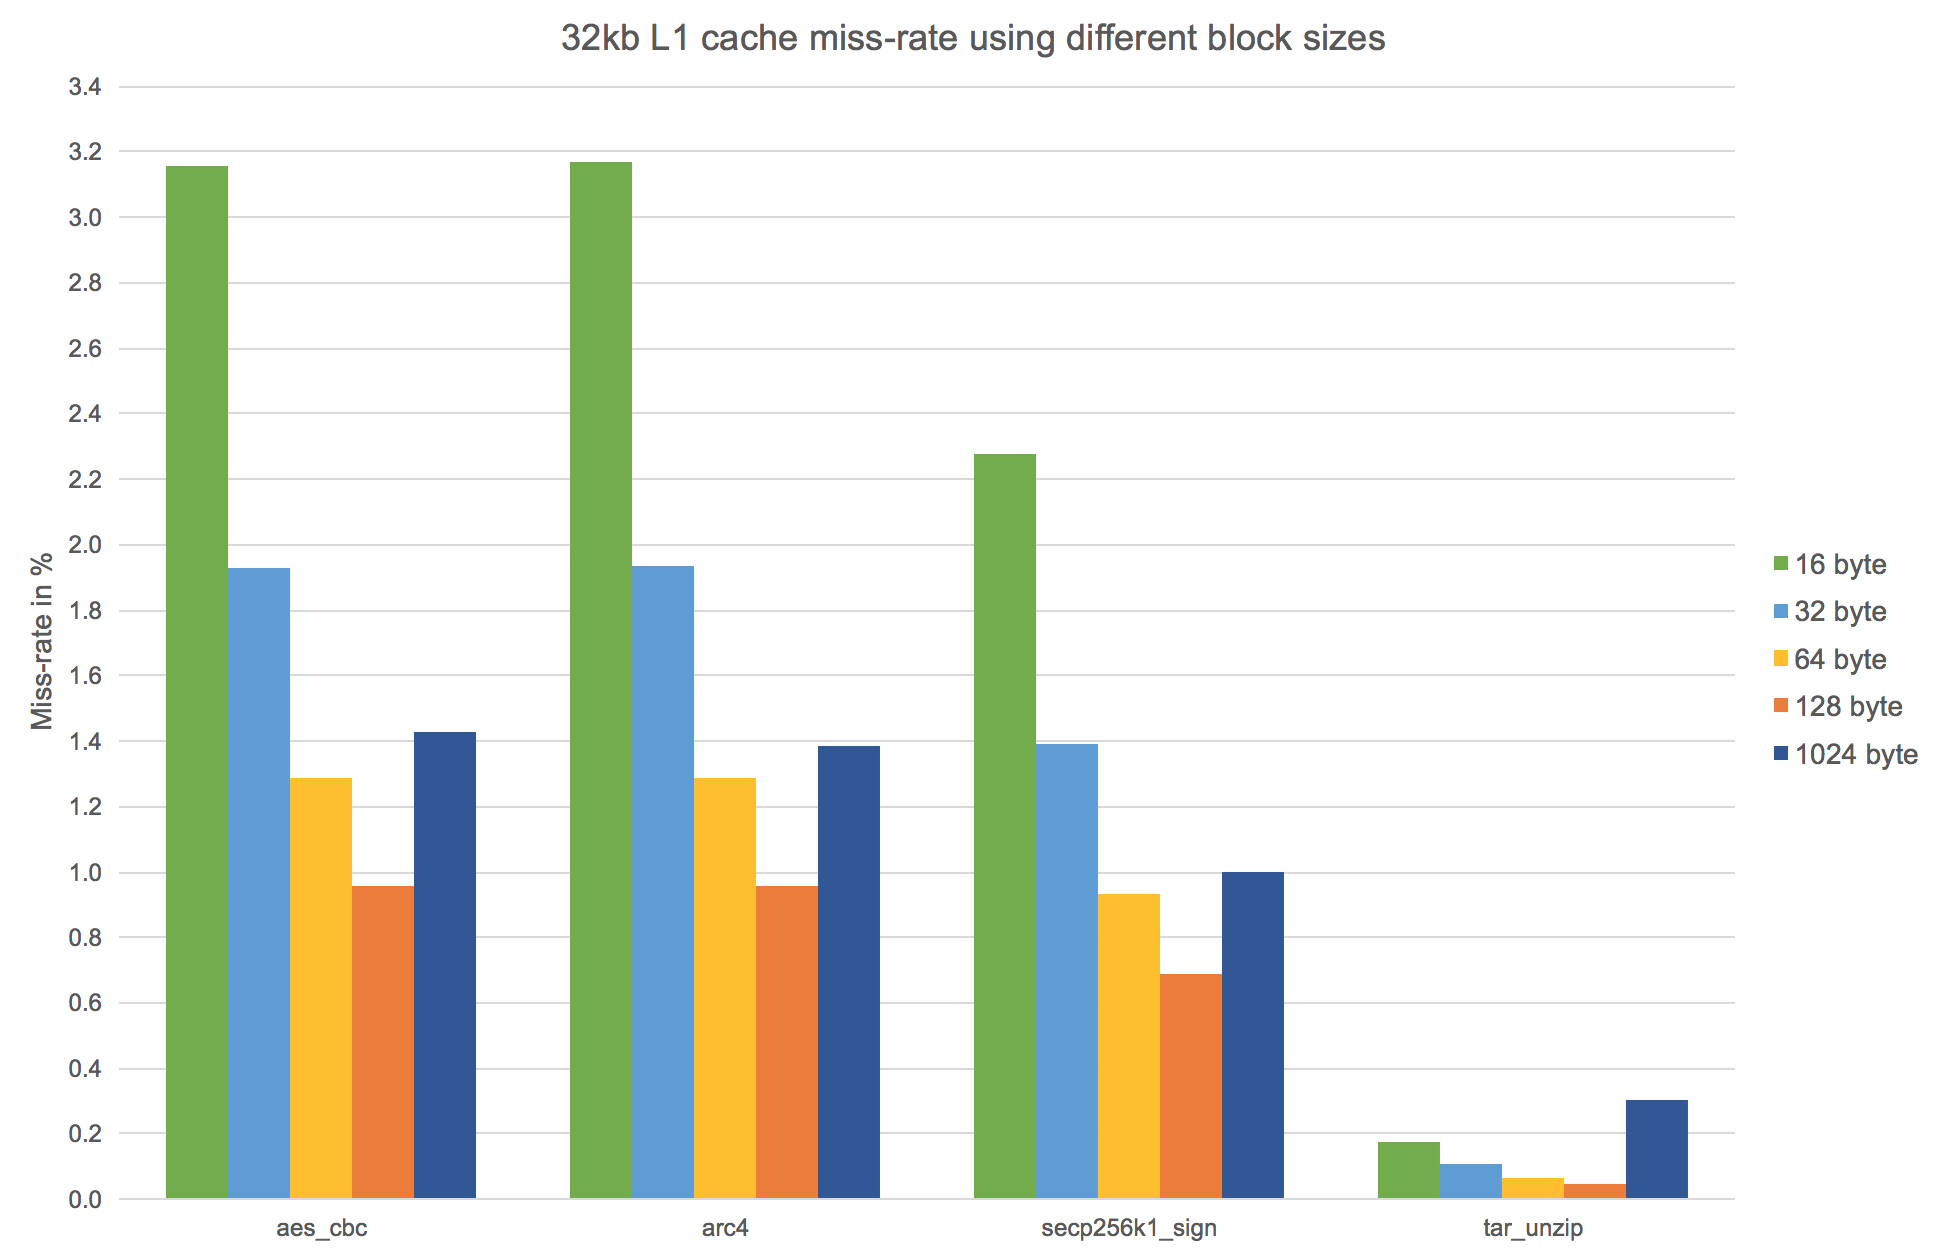
\includegraphics[width=\linewidth]{./figures/chart_diff_block_sizes.png}
		\caption{Advantage of spatial locality throughout all test cases.}
		\label{fig:diff_cache_block_sizes}
	\end{minipage}%
	\begin{minipage}{.5\textwidth}
		\centering
		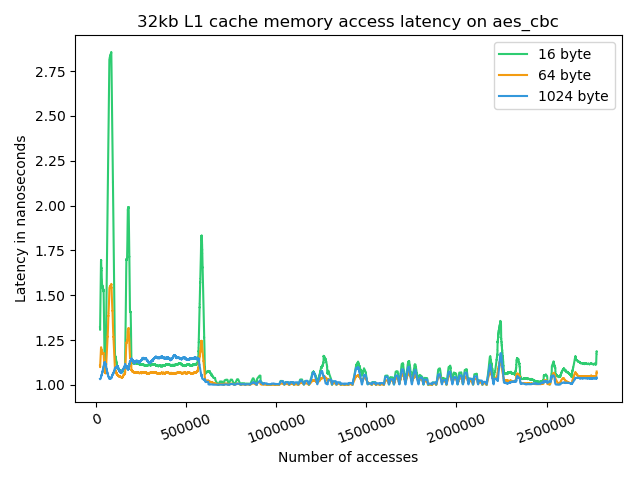
\includegraphics[width=\linewidth]{./figures/15-04-2018_14-55-50_aes_cbc-line_fetch_ns_rwindow=20000.png}
		\caption{Comparison of different cache block sizes on AES.}
		\label{fig:diff_cache_block_sizes_aes}
	\end{minipage}
\end{figure*}

In summary, set associative caches seem to outperform direct caches in practical applications. The advantage of set associative cache mapping arises through permit data to be stored in A-way different cache lines instead of forcing each memory address into one particular cache line. Imagine a cache that has no restraints about choosing a cache line aside from limited memory space. That means when data is fetched from main memory it can be placed in any unused block of the cache. When there is no more cache memory left, the eviction of cache lines is fully organized by a smart replacement algorithm. One can visualise it as a \textit{one set A-way cache}. This concept is called a \textit{fully associative cache}. Figure \ref{fig:fully_associative} illustrates theoretical performance gains using a full associative cache in comparison to a 4-way, 8-way and 16-way cache. The cache capacity was set to be 4 KiB and the block size 64 byte. Although this mapping principle has theoretical advantage over set associative caches, it is not feasible in practice due to its expensive implementation. Since we have no index, the etire address is used as a tag which increases the resulting cache size. Additionally, the data can be anywhere in the cache, so in worst case, we have to compare the tag of every cache line with the address tag. However, the huge amount of comparators needed led to the invention of set associative caches. The more ways, the higher the hardware costs. Thus, caches with a set associative of 4 to 16-ways are most widely used nowadays. 

Larger block sizes can take advantage of spatial locality by loading more data than actually needed, but also nearby addresses, into the cache \ref{section:cachemapping}. Figure \ref{fig:diff_cache_block_sizes} and \ref{fig:diff_cache_block_sizes_aes} both show measurements using different cache block sizes on a 32 KiB, 8-way cache with least recently used replacement algorithm. We observe that increasing the block size first lowers the cache miss-rate until a certain boundary is reached. A higher block size certainly decreases the number of sets possible due to a fixed cache capacity. In this example the cache with a block size of 64 byte has 64 cache sets, all containing eight different cache lines. A block size of 1024 byte produces only four sets containing eight cache lines each storing the block size, which means that on a cache-miss lots of data is fetched that never will be used before being evicted again. The most common block sizes used in microprocessors currently are 32 to 128 byte.  

\begin{figure}[!ht]
	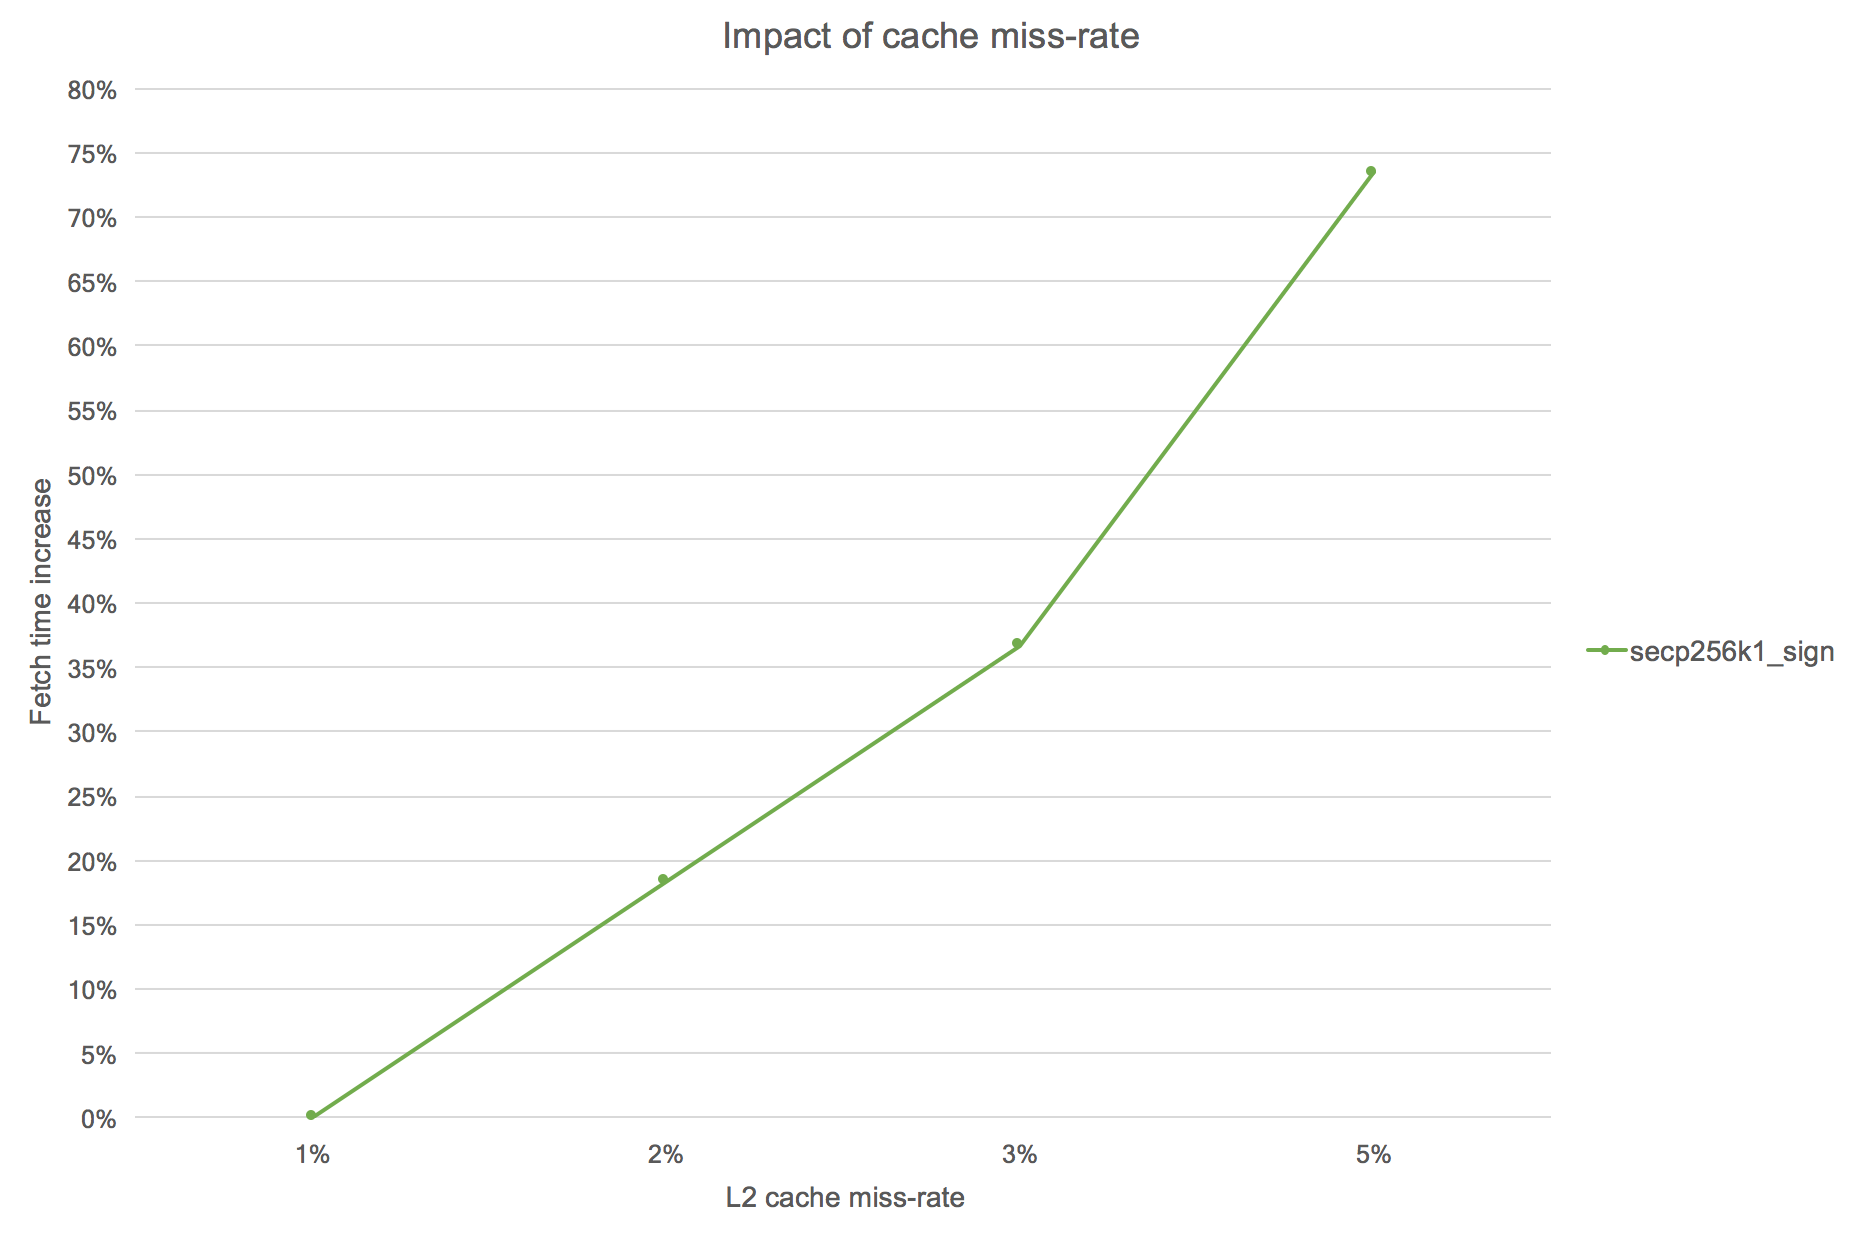
\includegraphics[width=\linewidth]{./figures/chart_impact_cache_miss-rate.png}
	\caption{Influence of miss-rate on data fetch time.}
	\label{fig:miss_rate_impact}
\end{figure}

To simulate the impact of the cache miss-rate on the overall performance, we now simulate a memory hierarchy consisting a L1 and L2 cache and main memory. We started with a L2 miss-rate of 1\% and increased its value to 5\% as shown in Figure \ref{fig:miss_rate_impact}. As mentioned before \ref{section:offlinesim}, the miss-rate has a huge impact on the overall systems performance. The data fetch time increases nearly 20\% on 1\% increase of the cache-miss rate. 

\subsubsection{Conclusion}

In review, it is obvious that microprocessor architectures focus on having memory content as near to the execution unit as possible, the time it is needed. We observed that a small improvement on the cache miss-rate can result in drastical performance gains to the overall system. To archieve the lowest miss-rate possible, microarchitectures make use of various principles like spatial and temporal locality, as well as smart replacement algorithms and cache hierarchies. A repository of this work can be found here \cite{misc:cachesim2018}.

\onecolumn
\pagebreak
\twocolumn
\bibliographystyle{plain}
\bibliography{bibliography}
%\nocite{*}
\end{document}
